\section{Supplementary Material}

\subsection{Background} \label{sup:background}

In the domain of experimental evolution, William Ratcliff and collaborators imposed a selective pressure for hydrodynamic settling on Baker's yeast and observed, in response, the emergence of a multicellular snowflake morphology in which parent and daughter cells remained tethered \citep{ratcliff2014experimental}.
With this system, they showed that multicellular life history can arise from a single mutation and demonstrated that unicellular bottlenecking of lineages implicitly arises as an inherent geometric consequence of the snowflake morphology \citep{ratcliff2015origins}.
Under extreme settling selection pressure, they observed the emergence (and, encumbered by free riders, subsequent collapse) of altruistic behavior in which extracellular DNA and proteins released under elevated apoptosis rates scaffolds the formation of multi-group collectives \citep{gulli2019evolution}.
Separately, incomplete cell separation mediated by the same mutational pathway has also been observed to evolve in response to selection for extracellular sucrose digestion at low population densities \citep{koschwanez2013improved}.

A wealth of mathematical models spanning both reductive and agent-based approaches have been developed to describe evolution of multicellularity and cellular specialization \cite{hanschen2015evolutionary}.
Recent work by Staps and collaborators exemplifies the increasing mechanistic nuance of contemporary computational models.
They present a mechanistic, agent-based system in which cells evolve weights for a Boolean gene regulatory network with two inputs (representing environmental state), two hidden nodes (representing regulatory state), and two outputs that control reproduction rate and probability of dissociation from or association into a group (representing gene products).
Evolutionary runs reveal how ecological conditions, such as predation pressure, constraints on diffusion of nutrients/waste, and changing environmental conditions, influence multicellular evolutionary outcomes with respect to group size, group lifespan, group fertility, and cell fate \citep{staps2019emergence}.
Staps et al. identify further augmentation of the mechanistic capabilities of their agents --- particularly the capacity to establish explicit spatial spatial structure within groups and sense local state --- as a compelling target for future work.

Heather Goldsby and collaborators' deme-based work is illustrative of the artificial life approach, where focal structures and processes realize conceptual analogy to (but not necessarily direct representation of) biological reality.
In this string of studies, spatially-segregated pockets of cells (``demes'') compete for space in a fixed-size population of demes.
Individual cells are controlled by self-replicating Avida-style computer programs with special instructions that allow them to interact with their environment and with neighboring cells.
The free-form paradigm of the genetic programming substrate, theoretically capable of performing arbitrary computation, enables the evolution of agents exhibiting the advanced behavioral capacities proposed by Staps et al., albeit in a manner without direct mechanistic analogy to biological cells.
Two modes of reproduction are defined under the deme model: within-deme and deme-founding.
In the first, a cell copies itself into a neighboring toroidal tile within its deme.
In the second, a deme slot is cleared in the deme population then seeded with a single cell from the parent deme.
Cells grow freely within demes, but deme fecundity depends on the collective profile of computational tasks (e.g., logic functions) performed within the deme.
This setup mirrors the dynamics of biological multicellularity, in which cell proliferation may either grow an existing multicellular body or spawn a new multicellular body.
Notably, when task-switching costs are applied Goldsby et al. have observed the evolution of division of labor and extensive functional interdependence within demes \citep{goldsby2012task}.
When mutagenic side-effects are applied Goldsby et al. have observed the evolution of germ-soma differentiation \citep{goldsby2014evolutionary}.

\subsection{Resource Collection Process} \label{sup:resource_collection_process}

Resource appears at a single point then spreads outwards update-by-update in a diamond-shaped wave.
The expanding wave halts at a predefined limit.
Cells must enter an ``activated'' state to harvest resource as it passes overhead.
The cell at the starting position of a resource wave is automatically activated, and will propagate the activation signal to neighboring cells in the same hereditary group.
The newly activated cells, in turn, activate their own neighbors registered to the same hereditary group.
Neighbors registered to other hereditary groups do not activate.
Each cell, after sending the activation signal, enters a temporary quiescent state.
In this manner, cells sharing a hereditary group track and harvest an expanding resource wave.
The rate of resource collection for a cell is determined by the size and shape of of its hereditary group;
small or fragmented hereditary groups will frequently miss out on resource as it passes by.

Resource waves have a limited extent.
Cells that activate outside the extent of a resource wave collect no resource.
A long quiescent period ensures that erroneously activated cells miss several subsequent opportunities to collect resource and therefore will tend to collect resource at a slower rate.
In this manner, ``Goldilocks'' --- not to small and not too big --- signaling networks enjoy superior fitness.
On L0 under the ``nested'' condition, resource waves extend a radius of two toroidal tiles.
On the apex level (L0 under the ``flat'' condition and on L1 under the ``nested'' condition) they extend a radius of six toroidal tiles.
On each level, activated cells netted $+0.2$ resource from a resource wave, but did not collect any resource outside the extent of the resource wave.

Resource wave starting points (seeds) are tiled over the toroidal grid from a randomly chosen starting location such that the extents of the resource waves do not overlap.
All resource waves begin and proceed synchronously;
when they complete, the next resource waves are seeded.
This process provides efficient, spatially-uniform, distributed selection for ``Goldilocks'' hereditary groups.

Cells control the size and shape of their hereditary group through strategic reproduction.
Three choices are afforded: whether to reproduce at all, where among the four adjoining tiles of the toroidal grid to place their offspring, and whether the offspring should be registered to the parent's hereditary group or be given a random hereditary ID (in the range 1 to $2^{64} - 1$).
The probability of hereditary group collision is miniscule: $60 \times 60 \times 2^{20}$ (the grid dimensions times the number of simulation updates) independent hereditary group IDs will collide with probability less than $1 \times 10^{-9}$.
No guarantees are made about the uniqueness of a newly-generated hereditary group ID, but chance collisions are vanishingly rare.

In addition to hereditary group-based resource collection, we provide a uniform inflow of $+0.0051$, sufficient for one reproduction approximately every thousand updates.

\subsection{Hereditary Group Life Cycle} \label{sup:hereditary_group_life_cycle}

Mature hereditary groups enjoy a considerable advantage over fledgling propagules.
Because of the isometric scaling relationship between surface area and perimeter, cooperating hereditary groups can marshal more resource at their periphery.
In addition, because of their greater surface area, mature hereditary groups are able to seed resource-wave events and collect resource at a higher per-cell rate.

In order to ensure hereditary group turnover and facilitate hereditary group propagation, we impose a timed phase-out of somatic reproduction and resource wave harvests.
For each cell, we track a hereditary group generation counter at each resource wave level.
At the genesis of a new hereditary group, these counters are set to zero.
Daughter cells that expand a hereditary group's soma are initialized to a counter value one greater than their parent.
Additionally, all hereditary generation counters are incremented every 512 updates to ensure that soma ages even in the absence of reproduction.
When a cell's hereditary group generation counter reaches 1.5 times the wave radius of its level, it can no longer produce somatic daughter cells.
Then, after two additional counter steps, cells lose their ability to seed resource wave events and collect resource.
Thus, as hereditary groups age over time, their constituent cells lose the ability regenerate somatic tissue and then, soon after, to collect resource.
To prevent complete stagnation in the case where all cells' hereditary group generation counters expire we provide a uniform inflow of $+0.0051$, sufficient for one reproduction approximately every thousand updates.

Interaction between nested hereditary groups produces a notable selective byproduct.
Because smaller, L0 hereditary groups tend to have intrinsically shorter lifespans, in order to achieve the full potential productive somatic lifespan of a larger, L1 hereditary group its constituent small hereditary groups must be intermittently regenerated.
Otherwise, the soma's capacity to seed resource-wave events and to collect resource will be prematurely lost once its constituent smaller, L0 hereditary groups expire.

This aging scheme's design ultimately stems from a desire
\begin{enumerate}
\item to facilitate evolution through regular turnover of emergent individuals and
\item to scaffold workable propagation for primitive cellular strategies while furnishing opportunities for more sophisticated adaptations to the imposed life cycle constraints.
\end{enumerate}
However, in some sense the aging scheme is heavy-handed, in effect enforcing rather than enabling a birth-death life cycle.
The evolutionary basis of aging and mortality --- in particular, the possibility of intrinsic evolutionary adaptations promoting these phenomena in addition to extrinsic factors  --- remains an active topic of scientific discussion \cite{baig2014evolution}.
In future work, we are interested in evaluating the outcomes of relaxing constraints of this aging scheme under different evolutionary conditions (such as cosmic ray mutations or irregular population structure) in light of theory attributing mortality and aging to evolvability, mutational accumulation, and costly somatic maintenance.

\subsection{Cell-Level Organisms} \label{sup:cell_level_organisms}

SignalGP programs are collections of independent procedural functions, each equipped with a bit-string tag \cite{lalejini2018evolving}.
A function is triggered by a signal with affinity that maximally and sufficiently matches its tag.
(A binding threshold of 0.1 was used in these experiments).
Signals may be generated by the environment, received as messages from other agents, or triggered internally by function execution.
Signals, and the ensuing chains of procedural execution they give rise to, are processed pseudo-concurrently by 24 virtual CPU cores.
Figure \ref{fig:signalgp-dishtinygp}\textbf{(A)} schematically depicts a single SignalGP instance.

In this work, we include a regulatory extension to the SignalGP system \cite{lalejini2021tag}.
During runtime, instructions may increase or decrease each tagged function's intrinsic tendency to match with --- and activate in response to --- tagged queries.
Intrinsic tag-to-tag match distances $m$ are modulated by a regulator value $r$ (baseline, 1.0) to become $r + r \times m$.
This scheme allows a function to be upregulated such that every query activates that function (e.g., $r = 0$) or no query activates that function (e.g., $r = \texttt{inf}$).
These regulation settings are heritable during reproduction but automatically decay after a number of updates determined when they are set.

To allow cells to protect themselves form potentially antagonistic interactions with their neighbors, we filter intercellular messages through a tag-matching membrane.
At runtime, cells can embed tags in this membrane that either admit or repel incoming messages.
Messages that do not match with a membrane tag are repelled.
A message, for example, that would activate a SignalGP function containing an apoptosis instruction could be rejected while other messages are accepted.
Tags embedded in this membrane automatically decay and may also be regulated.
We also filter messages between hardware instances within the same cell through a tag-matching membrane, but the default behavior for messages with unmatched tags is admission rather than rejection.

Previous work evolving digital organisms in grid-based problem domains has relied on a single computational instance which designates a direction to act in via an explicit cardinal ``facing'' state or output \cite{goldsby2014evolutionary, goldsby2018serendipitous, grabowski2010early, biswas2014causes, lalejini2018evolving}.
Under this paradigm, a large portion of genotype space encodes behaviors that are intrinsically asymmetrical with respect to absolute or relative (depending on implementation) cardinal direction.
However, in grid-based tasks, directional phenotypic symmetry is generally advantageous.
That is --- in the absence of a polarizing external stimulus --- successful agents generally behave uniformly with respect to each cardinal direction of the grid.
In this work, each cell employs four instances of SignalGP hardware: one ``facing'' each cardinal direction.
These computational instances all execute the same SignalGP program but are otherwise decoupled and may follow independent chains of execution and develop independent regulatory states.
Instances within a cell execute round robin step-by-step in an order that is randomly drawn at the outset of each update.

Genetic encodings that exploit problem-domain symmetries are known to promote evolvability and --- ultimately --- evolved solution quality \cite{clune2011performance, cheney2014unshackling}.
We submit that this directional hardware replication protocol likely increases the fraction of genotype space that encodes cardinally-symmetric phenotypes and therefore better facilitates the evolution of high-fitness phenotypes.
In further work, we look forward to exploring the evolvability and solution quality implications of this new approach.

The single SignalGP program that is mirrored across the cell's computational instances represents the cell's genome.
Mutation, with standard SignalGP mutation parameters as in \cite{lalejini2018evolving}, is applied to 1\% of daughter cells at birth.
In addition, genomes encode the bitstrings associated with environmental events.
These bitstrings evolve at a per-bit mutation rate equivalent to the bitstring labels of SignalGP functions.

Instances within a cell may send intracellular messages to one another or intercellular messages to a neighboring cell.
Intercellular messages are received by the SignalGP instance that faces the sending cell.
Figure \ref{fig:signalgp-dishtinygp}\textbf{(B)} schematically depicts the configuration of the four SignalGP instances that constitute a single DISHTINY cell as well as the instances of neighboring cells that receive extracellular messages from the focal cell.

\subsection{Standard SignalGP Instruction Library} \label{sup:standard_instruction_library}

The default SignalGP instruction set defines a number of generic arithmetic, logic, utility, and program flow instructions \cite{lalejini2018evolving}.
We include these instructions in our experiment's instruction library.

To counteract crowding of the mutational landscape by the volume of custom instructions provided, a second identical copy of each standard SignalGP instruction was included in the library.

\begin{itemize}
\item \textbf{Increment}
Increment value in a designated register.
\item \textbf{Decrement}
Decrement value in a designated register.
\item \textbf{Not}
Logically toggle value in a designated register.
\item \textbf{Add}
Add values from two designated registers into a third designated register.
\item \textbf{Subtract}
Subtract values from two designated registers into a third designated register.
\item \textbf{Multiply}
Multiply values from two designated registers into a third designated register.
\item \textbf{Divide}
Divide values from two designated registers into a third designated register.
\item \textbf{Modulus}
Calculate the modulus from two designated registers and place result into a third designated register.
\item \textbf{Test Equal}
Compare values in two designated registers and place equality result into a third designated register.
\item \textbf{Test Non-equality}
Compare values in two designated registers and place opposite equality result into a third designated register.
\item \textbf{Test Less}
Compare values in two designated registers and place less-than result into a third designated register.
\item \textbf{If}
If a designated register is non-zero, proceed.
Otherwise, skip block.
\item \textbf{While}
While a designated register is non-zero, loop over a program block.
Otherwise, skip block.
\item \textbf{Countdown}
While a designated register is non-zero, loop over a program block and decrement the value in the designated register.
Otherwise, skip block.
\item \textbf{Close}
If a preceding program block is, close it.
\item \textbf{Break}
Break to the end of the current program block.
\item \textbf{Call}
Call the SignalGP program module that best matches instruction's affinity.
\item \textbf{Return}
If possible, return from the current function.
\item \textbf{Set Memory}
Set a designated register's value to hard-coded memory value.
\item \textbf{Set True}
Set a designated register's value to true (1.0).
% terminal
\item \textbf{Copy Memory}
Copy the value of a designated register to a second designated register.
\item \textbf{Swap Memory}
Swap the values of two designated registers.
\item \textbf{Input}
Copy a designated element of input memory into a designated register.
\item \textbf{Output}
Copy to a designated element of output memory from a designated register.
\item \textbf{Commit}
Copy a designated register into a designated element of global memory.
\item \textbf{Pull}
Copy a designated element of global memory into a designated register.
\item \textbf{Fork}
Fork a new thread with the SignalGP program module that best matches the instruction's affinity.
\item \textbf{Terminate}
Terminate the current thread.
\item \textbf{Nop}
No operation.
\item \textbf{RNG Draw}
Draw a random value between 0.0 and 1.0 from random number generator and store result in a register.
\item \textbf{Set Regulator}
Set the program module regulator that best matches (without regulation) the instruction's affinity to the value of a designated register.
\item \textbf{Set Own Regulator}
Set the program module regulator of the currently-executing program module to value of a designated register.
\item \textbf{Adjust Regulator}
Adjust the program module regulator of the program module that best matches (without regulation) the instruction's affinity a designated fraction toward a designated register's value.
\item \textbf{Adjust Own Regulator}
Adjust the program module regulator of the currently-executing program module a designated fraction toward a designated register's value.
\item \textbf{Extend Regulator}
Adjust the program module regulator decay timer of the program module that best matches (without regulation) the instruction's by a designated register's value.
\item \textbf{Sense Regulator}
Copy the program module regulator value of the program module that best matches (without regulation) the instruction's affinity into a designated register.
\item \textbf{Sense Own Regulator}
Copy the program module regulator value of currently-executing program module into a designated register.
\end{itemize}

\subsection{Custom Instruction Library} \label{sup:custom_instruction_library}

We define a number of custom instructions to allow evolving programs to sense and interact with their environment, through mechanisms including
\begin{itemize}
\item reproduction,
\item resource sharing,
\item hereditary group ID sensing,
\item apoptosis,
\item intracellular messaging, and
\item intercellular messaging.
\end{itemize}

We provide an listing of our experiment's instruction library below.

Instructions that involve an extracellular neighbor default to the cell that the executing SignalGP instance is facing.
To ensure a founding crop of viable individuals, apoptosis and program flow instructions in the initial randomly-generated population were replaced with no-op instructions.
However, these instructions were allowed to mutate in to genomes freely once evolutionary runs began.

\begin{itemize}
\item \textbf{Send Intracellular Message}
Send a message to a single other SignalGP instance within the cell specified by a designated register's value.
\item \textbf{Broadcast Intracellular Message}
Send a message to all SignalGP instances within the cell, excluding self.
\item \textbf{Put Internal Membrane Gatekeeper}
% bringer / blocker
Place a tag in the internal membrane that, depending on insertion order, admits or blocks incoming internal messages it matches with.
\item \textbf{Send Intercellular Message}
Send a message to a single cellular neighbor.
\item \textbf{Broadcast Intercellular Message}
Send a message to all cellular neighbors.
\item \textbf{Put External Membrane Gatekeeper}
% bringer / blocker
Place a tag in the external membrane that, depending on insertion order, admits or blocks incoming external messages it matches with.
\item \textbf{Set External Membrane Regulator}
Set the regulation of the gatekeeper in the external membrane that best matches (without regulation) the instruction's affinity to the value of a designated register.
\item \textbf{Adjust External Membrane Regulator}
Adjust the regulation of the gatekeeper in the external membrane that best matches (without regulation) the instruction's affinity a designated fraction toward a designated register's value.
\item \textbf{Sense External Membrane Regulator}
Copy the regulation value of the program module that best matches (without regulation) the instruction's affinity into a designated register.
\item \textbf{Activate Intercellular Inbox}
Mark the intercellular inbox to accept messages.
At cell birth, the inbox is deactivated.
\item \textbf{Deactivate Intercellular Inbox}
Mark the intercellular inbox to decline messages.
\item \textbf{Share Resource}
Send a proportion of the cell's stockpiled resource to a neighboring cell.
One instruction defaults to sending a large proportion of available resource (50\%) to the neighboring cell.
A second instruction defaults to sending a small proportion of available resource (5\%) to the neighboring cell.
The proportion of available resource can be adjusted by a register-based argument.
\item \textbf{Set Stockpile Sharing Reserve}
Designate a quantity of stockpiled resource as ineligible for sharing.
The amount may be modified by a register-based argument.
\item \textbf{Clear Stockpile Sharing Reserve}
Designate all stockpiled resource as eligble for sharing.
\item \textbf{Restrict Outgoing Shared Resource}
Reduce outgoing sharing efficacy.
Unsent resource is retained by the sending cell (with no resource lost).
The fraction reduced is determined by a register-based argument.
\item \textbf{Restrict Incoming Shared Resource}
Reduce incoming sharing efficacy.
Declined resource is retained by the sending cell (with no resource lost).
The fraction reduced is determined by a register-based argument.
\item \textbf{Reproduce}
Attempt to spawn a child cell in a particular direction, paid for out of the parent cell's resource stockpile.
If sufficient resource is not available in the cell's stockpile, no resource is action is taken.
Variants of this instruction are defined for each hereditary group ID inheritance level: from endowing the daughter cell with the parental hereditary group IDs across all levels, to endowing the daughter cell with a new level-one hereditary group ID but the parent's level-two hereditary group ID, to endowing the daughter cell with all-new hereditary group IDs.
If a hereditary group generation counter limit has been reached, reproduction is simply attempted at the next highest level; even with hereditary group generation counters maxed out, cells may generate offspring with all-new hereditary group IDs.
\item \textbf{Pause Reproduction}
Pause cellular reproduction in a single direction for the remainder of the current update and for the entire next update.
Variants of this instruction pause reproduction at a certain hereditary grouping level or across all hereditary group inheritance levels.
\item \textbf{Set Stockpile Reproduction Reserve}
Designate a quantity of stockpiled resource as ineligible for use to reproduce.
The amount may be modified by a register-based argument.
\item \textbf{Clear Stockpile Sharing Reserve}
Designate all stockpiled resource as eligible for use to reproduce.
\item \textbf{Apoptosis}
The cell is killed at the end of the current update.
\item \textbf{Designate/Revoke Heir} A dying cell's own stockpile is split evenly among neighboring cells that are designated at the time of death.
On apoptosis, 50\% of the reproduction cost to establish a cell is also split between designated neighboring cells.
These instructions mark or un-mark a neighbor as a heir.
\item \textbf{Increase Hereditary Group Generation Counter}
Increases the cell's hereditary group generation counter.
The amount the cell's generation counter is increased by can be adjusted by register-based argument.
\item \textbf{Query Own Stockpile}
Sets a designated register to the amount of resource present in the cell's stockpile.
\item \textbf{Query Own Hereditary Group Generation Counter}
This instruction sets a designated register to the value of the cell's hereditary group generation counter.
A variant of this instruction is provided for each hereditary group level.
\item \textbf{Query ``Is Neighbor Live?''}
This instruction sets a designated register to 1 if the neighboring tile contains a live cell and 0 otherwise.
\item \textbf{Query ``Is Neighbor My Cellular Child?''}
This instruction sets a designated register to 1 if the neighboring cell is the daughter of the querying cell and 0 otherwise.
\item \textbf{Query ``Is Neighbor My Cellular Parent?''}
This instruction sets a designated register to 1 if the neighboring cell is the parent of the querying cell and 0 otherwise.
\item \textbf{Query ``Does Neighbor's Hereditary Group ID Match Mine?''}
This instruction sets a designated register to 1 if the neighboring cell has the same hereditary group ID as the querying cell and 0 otherwise.
A variant of this instruction is provided for each level of hereditary grouping.
\item \textbf{Query ``Does Neighbor's Hereditary Group ID Descend From Mine?''}
This instruction sets a designated register to 1 if the neighboring cell's highest-level hereditary group ID is different from the querying cell's highest-level hereditary group ID, but is descended from the querying cell's hereditary group ID via an explicit propagule-generating reproduction call.
This instruction allows a querying cell to sense whether its neighbor is a member of a hereditary group that is a propagule of the querying cell's hereditary group.
\item \textbf{Query ``Does My Hereditary Group ID Descend From Neighbor's?''}
This instruction sets a designated register to 1 if the querying cell's highest-level hereditary group ID is different from the neighboring cell's highest-level hereditary group ID, but is descended from the neighboring cell's hereditary group ID  via an explicit propagule-generating reproduction call.
This instruction allows a querying cell to sense whether it is a member of a hereditary group that is a propagule of the neighboring cell's hereditary group.
\item \textbf{Query ``Is Neighbor Poorer?''}
This instruction sets a designated register to 1 if the querying cell's resource stockpile is larger than the neighboring cell's.
\item \textbf{Query ``Is Neighbor Older?''}
This instruction sets a designated register to 1 if the querying cell's cell age is less than the neighboring cell's.
\item \textbf{Query ``Is Neighbor Expired?''}
This instruction sets a designated register to 1 if a neighboring cell's hereditary group generation counter has exceeded the expiration threshold.
\item \textbf{Query Neighbor's Hereditary Group ID}
This instruction sets a designated register to the neighbor's hereditary group ID.
A variant of this instruction is provided for each hereditary grouping level.
\item \textbf{Query Neighbor's Stockpile}
This instruction sets a designated register to the amount of resource present in the neighbor's stockpile.
\end{itemize}

\subsection{Environmental Cue Library} \label{sup:environmental_cue_library}

Event-driven sensing has been shown to enable evolution of SignalGP programs that more successfully react to  environmental state \cite{lalejini2018evolving}, so we supplement our instruction-based sensors with event-based input.
Every eight updates, a subset of environmental events are triggered on each SignalGP hardware based on current local environmental conditions.
The activating affinity of each event is genetically-encoded as part of the program currently executing on the hardware.
We provide a listing of our experiment's event library in supplementary material \ref{sup:environmental_cue_library}.

\begin{itemize}
\item \textbf{On Update}
This event is triggered every eight updates.
\item \textbf{Just Born}
This event is triggered once after a cell is born.
\item \textbf{Richer Neighbor}
This event is triggered if a neighbor cell has more stockpiled resource than the focal cell.
\item \textbf{Poorer Neighbor}
This event is triggered if a neighbor cell has less stockpiled resource than the focal cell.
\item \textbf{Facing Cellular Child}
This event is triggered if the SignalGP instance is facing a neighboring cell that is the querying cell's daughter.
\item \textbf{Facing Cellular Parent}
This event is triggered if the SignalGP instance is facing a neighboring cell that is the querying cell's parent.
\item \textbf{Neighbor's Hereditary Group ID Descends From Mine}
This event is triggered if the neighboring cell's highest-level hereditary group ID is different from the querying cell's highest-level hereditary group ID, but is descended from the querying cell's hereditary group ID via an explicit propagule-generating reproduction call.
This event allows a querying cell to sense whether its neighbor is a member of a hereditary group that is a propagule of the querying cell's hereditary group.
\item \textbf{My Hereditary Group ID Descends From Neighbor's}
This event is triggered if the focal cell's highest-level hereditary group ID is different from the neighboring cell's highest-level hereditary group ID, but is descended from the neighboring cell's hereditary group ID via an explicit propagule-generating reproduction call.
This event allows a neighboring cell to sense whether its neighbor is a member of a hereditary group that is a propagule of the neighboring cell's hereditary group.
\item \textbf{Neighbor's Hereditary Group ID Matches Mine}
This event is triggered if a SignalGP instance is facing a neighbor cell that shares its hereditary group ID.
A different event is provided for each level of hereditary grouping.
\item \textbf{Neighbor's Hereditary Group ID Does Not Match Mine}
This event is triggered if a SignalGP instance is facing a neighbor cell that does not share its hereditary group ID.
A different event is provided for each level of hereditary grouping.
\item \textbf{Hereditary Group Generation Counter Is Unexpired}
This event is triggered if a SignalGP instance's cell's hereditary group generation counter has not yet reached the expiration threshold.
A different event is provided for each level of hereditary grouping.
\item \textbf{Hereditary Group Generation Counter Is Expiring}
This event is triggered if a SignalGP instance's cell's hereditary group generation counter has not yet reached the threshold where somatic propagation capacity, but not resource accumulation capacity, is lost.
A different event is provided for each level of hereditary grouping.
\item \textbf{Hereditary Group Generation Counter Is Expired}
This event is triggered if a SignalGP instance's cell's hereditary group generation counter has not yet reached the threshold where both somatic propagation capacity and resource accumulation capacity are lost.
A different event is provided for each level of hereditary grouping.
\item \textbf{No-reward Resource Activation}
This event is triggered if a SignalGP instance's cell experiences a resource collection activation where no resource reward is achieved (e.g., the cell lies extent of the resource wave).
A different event is provided for each level of hereditary grouping.
\end{itemize}

\subsection{Evolutionary Conditions} \label{sup:treatments}

\pragmaonce

% adapted from https://tex.stackexchange.com/a/17491
\makeatletter
  \def\importpath{\import@path}
\makeatother


\begin{table*}[!htbp]
\begin{center}
\footnotesize
\caption{
Observed productivity at epoch 1 (mean $\pm$ S.D.).
}
\label{tab:productivity}

\begin{tabular}{l|c|c|c|c}%
\bfseries Measure
  & \bfseries Flat-Even
  & \bfseries Flat-Wave
  & \bfseries Nested-Even
  & \bfseries Nested-Wave
\csvreader[head to column names]{\importpath data/productivity.csv}{}
{\\\hline\Measure
  & \FlatEven
  & \FlatWave
  & \NestedEven
  & \NestedWave
}
\end{tabular}

\end{center}
\end{table*}


\pragmaonce

% adapted from https://tex.stackexchange.com/a/17491
\makeatletter
  \def\importpath{\import@path}
\makeatother

% \pragmaonce

% adapted from https://www.overleaf.com/learn/latex/Commands
\providecommand{\dissertationelse}[2]{%
% adapted from https://tex.stackexchange.com/a/33577
\ifdefined\DISSERTATION
#1
\else
#2
\fi
}


\begin{sidewaystable}
\begin{center}
\dissertationelse{\fontsize{9}{10}\selectfont}{\footnotesize}
\begin{tabular}{l|c|c|c|c|c|c|c|c}%
&\multicolumn{4}{c|}{Epoch 1}
&\multicolumn{4}{c}{Epoch 4}\\
\bfseries Measure
  & \bfseries Flat-Even
  & \bfseries Flat-Wave
  & \bfseries Nested-Even
  & \bfseries Nested-Wave
  & \bfseries Flat-Even
  & \bfseries Flat-Wave
  & \bfseries Nested-Even
  & \bfseries Nested-Wave
\csvreader[head to column names]{\importpath data/systematics.csv}{}
{\\\hline\Measure
  & \FlatEvenShort
  & \FlatWaveShort
  & \NestedEvenShort
  & \NestedWaveShort
  & \FlatEvenLong
  & \FlatWaveLong
  & \NestedEvenLong
  & \NestedWaveLong
}
\end{tabular}

\caption{
Systematics outcomes (mean $\pm$ S.D.)
}

\label{tab:systematics}
\end{center}
\end{sidewaystable}


In this work, we screened replicates conducted under combinations of two experimental conditions:
\begin{enumerate}
\item flat versus two nested hierarchical levels of hereditary grouping and
\item cooperative versus independent resource collection.
\end{enumerate}

The first experimental manipulation explores the effects of hierarchical nesting of kin-sensing and/or functional cooperation.
The second manipulation explores the effects of functional cooperation.

To enact the first manipulation, we compared the nested hierarchical hereditary grouping scheme described above with a single-level scheme with waves extending six toroidal tiles.
We also increased the resource wave reward to $+0.6$ to approximately match the observed resource inflow rate of the nested scheme.
To enact the second manipulation, we removed the resource wave reward and increased the uniform resource inflow rate to $+0.0175$ in order to approximately match the net inflow rate under the dual-level wave-based scheme.
Table \ref{tab:productivity} reports productivity observed under these different conditions.

We mix and match these experimental manipulations in three treatments:
\begin{enumerate}
\item one level with even resource (``Flat-Even''; in-browser simulation \url{https://hopth.ru/i}),
\item one level with wave-based resource (``Flat-Wave''; in-browser simulation \url{https://hopth.ru/j}),
\item two levels with even resource (``Nested-Even''; in-browser simulation \url{https://hopth.ru/k}), and
\item two levels with wave-based resource (``Nested-Wave''; in-browser simulation \url{https://hopth.ru/l}).
\end{enumerate}

We ran 40 replicates under each treatment condition.
Replicates were seeded with randomly generated SignalGP programs.
To conserve disk space, we divided evolutionary runs into 262144 ($2^{18}$) update epochs and collected data in 8096 ($2^{13}$) update snapshots between epochs.
All replicates ran at least one full epoch, and all comparisons between or within treatments are conducted at this time point.
However, most replicates (156/160) were able to run to four epochs during available compute time.
We screened for and conducted case studies at the latest available data for each replicate.
All reported case studies happen to be drawn from runs that completed 4 epochs of evolution.
Table \ref{tab:systematics} reports the systematics outcomes observed under each treatment at epoch 1 and at epoch 4.

All experiments took place on a traditional 60-by-60 toroidal grid, supporting a population of at most 3600 individual cells.

\subsection{Competition Experiments and Phenotype Assays} \label{sup:competition_assays}

We performed further experiments to develop case studies of evolved strains we manually screened from our evolutionary runs.
In these experiments, the most-abundant genotype was harvested from the end-state of evolutionary runs as the wild type strain.
We collected epigenetic state (i.e., regulatory settings) along with genetic state (i.e., SignalGP program and environmental-cue-to-tag mapping).
All further work with harvested strains was conducted under environmental conditions identical to that of the treatment they evolved in.

To analyze the relative fitness of knockout strains versus wild type, we seeded 20 $60 \times 60$ toroidal grids with ten cells of each strain, including epigenetic regulator state.
We ran competition experiments for the duration of one snapshot.
Seeded cells generally proliferated to completely fill the toroidal grid in the first quarter of the snapshot.
Competition experiment outcomes were determined by strains' relative cell populations within the grid at the end of the snapshot.

To perform phenotypic comparisons between knockout strains and wild type, we seeded ten cells of each strain onto separate $60 \times 60$ toroidal grids and then cultured them for the duration of one snapshot.

\subsection{Implementation} \label{sup:implementation}

We implemented our experimental system using the Empirical library for scientific software development in C++, available at \url{https://github.com/devosoft/Empirical} \citep{charles_ofria_2019_2575607}.
The code used to perform and analyze our experiments, our figures, data from our experiments, and a live in-browser demo of our system is available via the Open Science Framework at \url{https://osf.io/g58xk/}.
Most replicates finished within a day, but some took up to a week to complete.

\subsection{Reproductive Cooperation} \label{sup:reproductive-cooperation}

\begin{figure}[!htbp]
\begin{center}

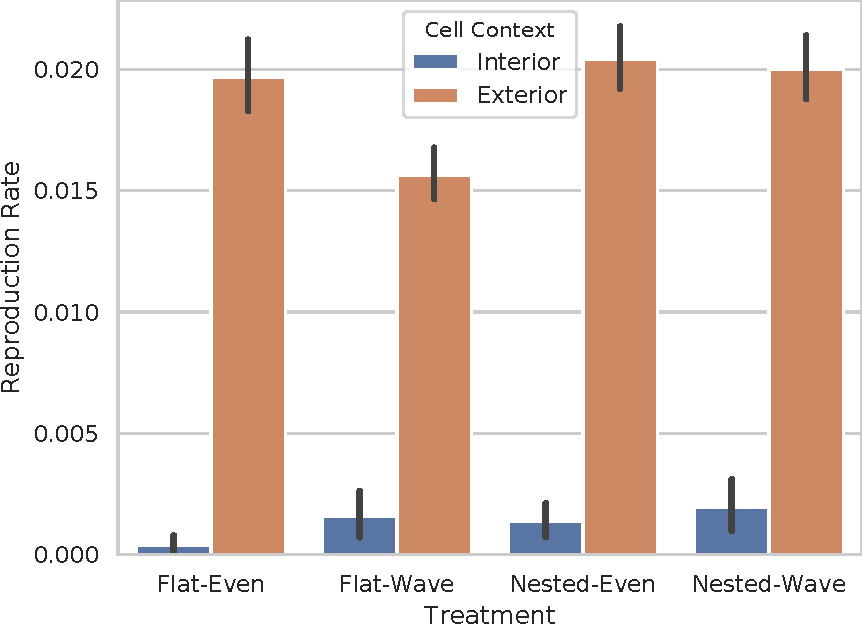
\includegraphics[width=\columnwidth]{img/reproduction/title=reproductive_labor_surrounded+_data_hathash_hash=2400d97af0b49a99+_script_fullcat_hash=d728fc498d889102+_source_hash=53a2252-clean+ext=}

\caption{
Cellular reproduction rates at the interior and exterior of apex-level hereditary groups.
Error bars indicate 95\% confidence.
}
\label{fig:reproduction_surrounded}
\end{center}
\end{figure}


\subsection{Resource Sharing} \label{sec:resource-sharing}

\begin{figure*}[!htbp]
\begin{center}

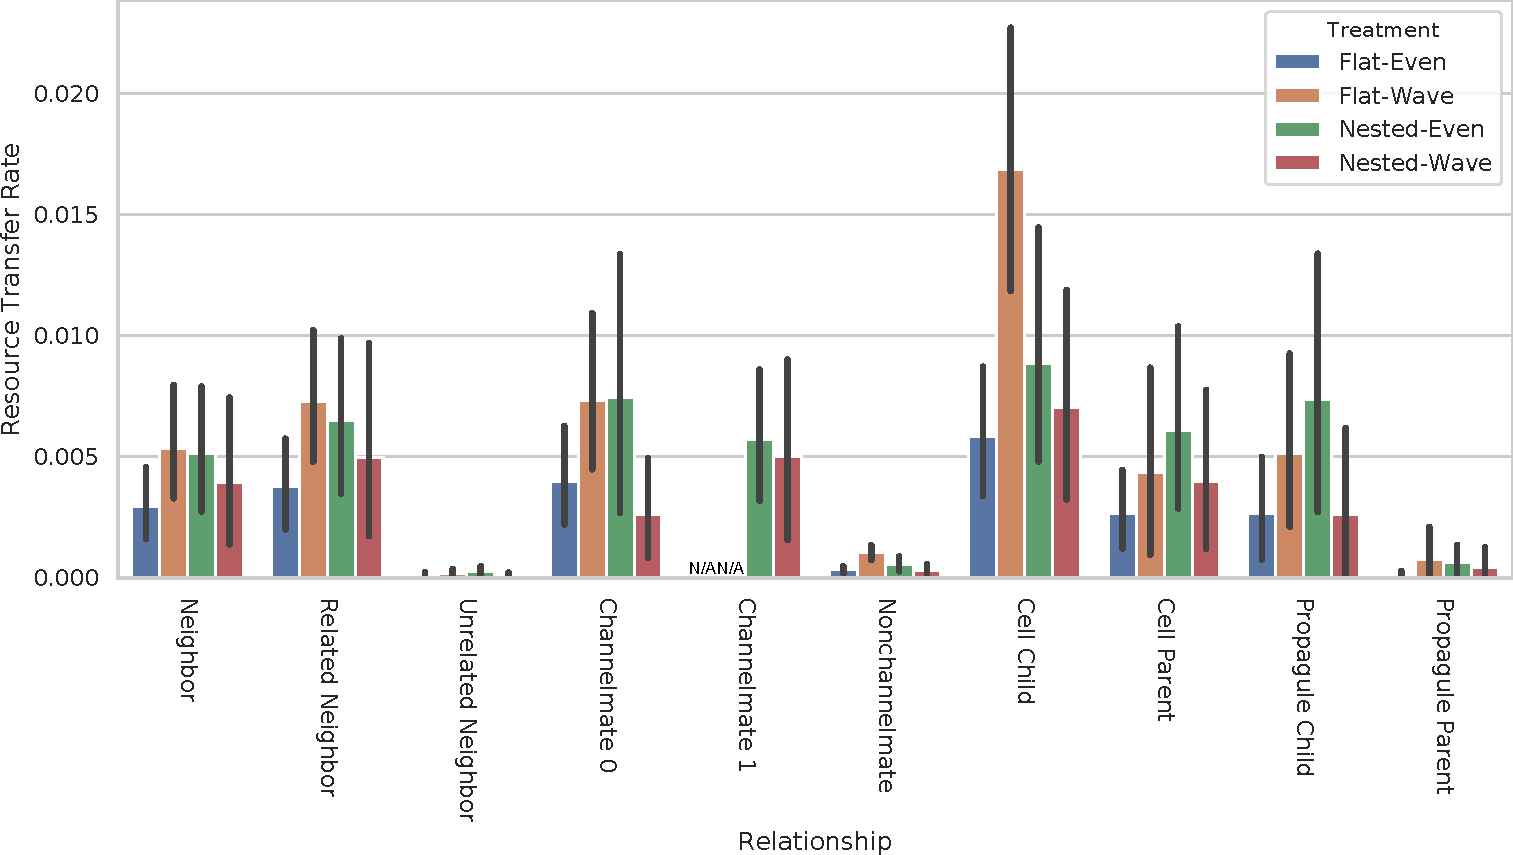
\includegraphics[width=\textwidth]{sharing/title=Resource_Transfer_Rate+_data_hathash_hash=ade957ec08284082+_script_fullcat_hash=e37b8d6f029c9f40+_source_hash=53a2252-clean+ext=}

\caption{
Resource sharing rates across donor-recipient relationships.
Neighbor describes any potential recipient cell.
Related neighbor describes a recipient cell that is a direct cellular progenitor or offspring of the donor, registered to a same hereditary group as the donor, or a member of a hereditary group that is a progenitor or offspring of the donor's.
Unrelated neighbors constitutes all other cells.
Channelmate refers to donor-recipient pairs that are registered to the same hereditary group.
Note that L1 groups are not defined in the flat treatment.
Non-channelmate recipients are not registered to any common hereditary groups with the potential donor.
Cell child and parent describe direct nuclear cell relationships between donor and recipient.
Finally, a propagule child relationship exists when a donor cell is a member of the apex-level hereditary group that directly begat the recipient cell's hereditary group.
A propagule parent relationship describes the reverse, when a recipient cell is a member of the apex-level hereditary group that directly begat the donor cell's hereditary group.
Error bars indicate 95\% confidence.
}
\label{fig:sharing}
\end{center}
\end{figure*}

\begin{figure*}[!htbp]
\begin{center}

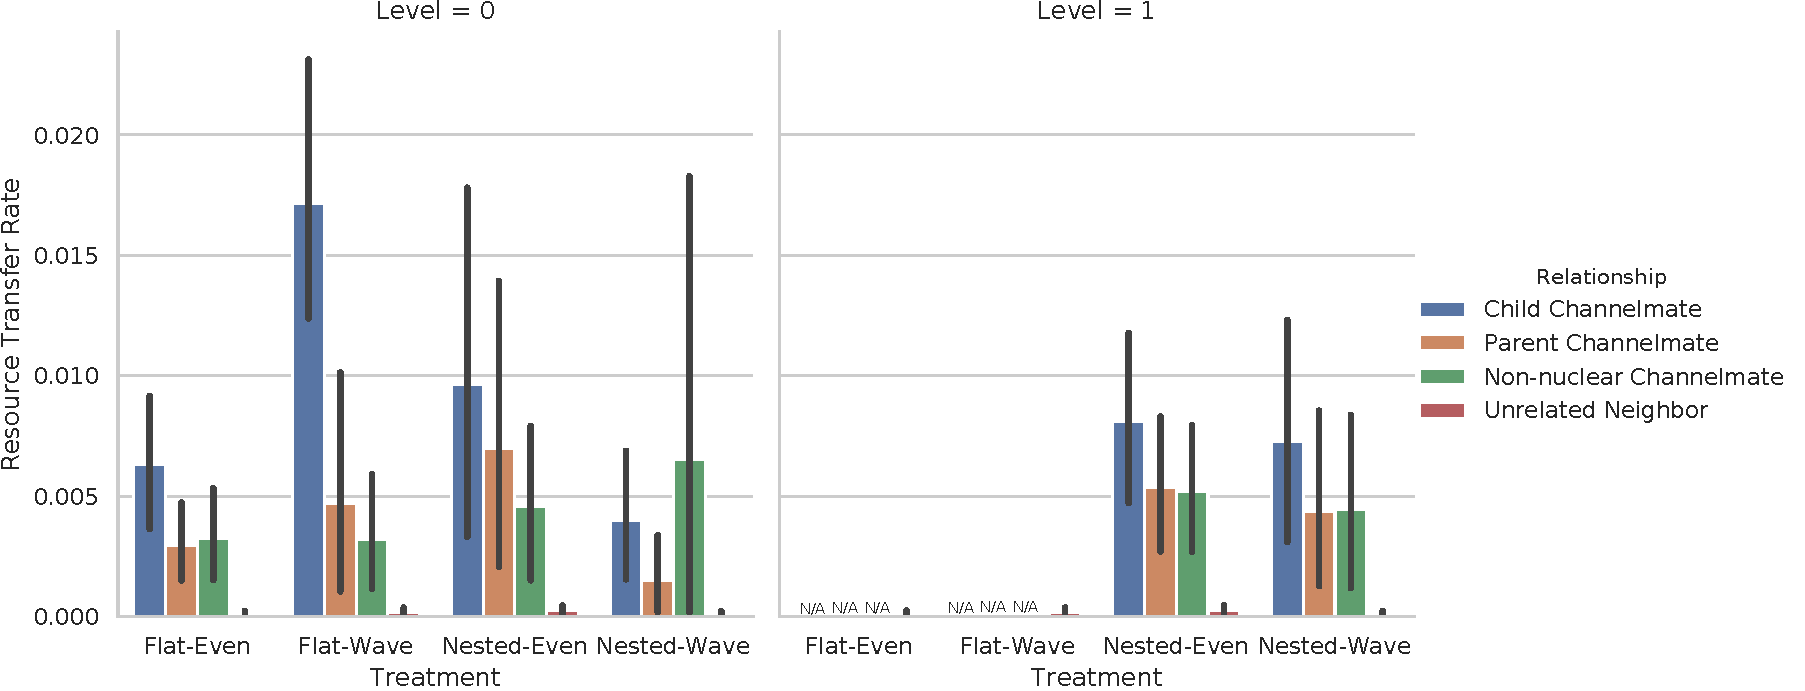
\includegraphics[width=\textwidth]{sharing/title=Resource_Transfer_Rate+_data_hathash_hash=2137e250b9d2b681+_script_fullcat_hash=86edbf4a4e5f34ed+_source_hash=53a2252-clean+ext=}

\caption{
Resource sharing to mutually exclusive sub-categories of hereditary group comrades: cellular child, cellular parent, and neither (``non-nuclear'').
Resource sharing to entirely non-related cells (no cell, hereditary group, or propagule relation) is included for comparison.
Note that L1 hereditary groups are not defined in either of the flat treatments.
Error bars indicate 95\% confidence.
}
\label{fig:sharing_channelmate}
\end{center}
\end{figure*}


Figure \ref{fig:sharing} overviews evolved resource sharing behavior across cellular contexts.

Replicates in the flat-wave treatment exhibit an especially elevated rate of resource sharing to cell children.
This could perhaps be due to an especial selective pressure to convey resource towards the group periphery.

In the Nested-Wave treatment resource was shared at a higher mean rate among L1 hereditary groups than L0 groups.
At face value, this observation appears counterintuitive: why should cells prefer to share with more distant relatives with only one hereditary ID in common as opposed to closer relatives with both hereditary IDs in common?
However, we believe it likely an artifact of replicates where L1 groups were composed of single-cell L0 groups (where no or very few opportunities for L0 resource sharing occurred).

Finally, under all treatments resource was transferred to hereditary group comrades at a significantly higher mean rate than to unrelated neighbors (non-overlapping 95\% CI).
This observation suggests that functional cooperation within hereditary groups might have been a common evolutionary outcome under all four treatments.
However, it could potentially be driven exclusively by resource-sharing between direct cellular kin.

Figure \ref{fig:sharing_channelmate} investigates this possibility by breaking within-group resource sharing apart by cellular kin relation.
In all four treatments, mean sharing to direct-kin hereditary group comrades was indeed greater than to other hereditary group comrades.
This could be due to an evolutionary incentive to favor direct cell kin over other hereditary comrades, group-level selection for asymmetric resource flow achieved by preferential sharing, or some combination of the two.
However, in all four treatments mean sharing to non-direct-kin hereditary group comrades was also significantly greater than resource sharing to unrelated neighbors (non-overlapping 95\% CI).
Thus, all four treatments appear to be sufficient to select for functional cooperation within hereditary groups.

\subsection{Case Study: Cell-Cell Messaging} \label{sec:intergroup}

% \pragmaonce

% adapted from https://www.overleaf.com/learn/latex/Commands
\providecommand{\dissertationelse}[2]{%
% adapted from https://tex.stackexchange.com/a/33577
\ifdefined\DISSERTATION
#1
\else
#2
\fi
}


\begin{figure}[!htbp]
\begin{center}
\begin{minipage}[t]{0.5\linewidth}


% \begin{minipage}[t]{\linewidth}
\centering
\hspace*{\fill}%
\begin{minipage}[t]{0.05\linewidth}
\vspace{0pt} % for alignment
\rotatebox{90}{Messaging}%
\end{minipage}%
\hfill
\begin{minipage}[t]{0.45\linewidth}
\centering
\vspace{0pt} % for alignment
\adjincludegraphics[width=\textwidth, trim={{.66\width} {.66\width} {.0\width} {.0\width}}, clip]{img/knockout/intermessaging-intergroup_border/wildtype/seed=1+title=directional_messaging_viz+treat=resource-wave__channelsense-yes__nlev-two+update=7168+_data_hathash_hash=3895dfa0dd602b4c+_script_fullcat_hash=6b7e0389992dd616+_source_hash=53a2252-clean+ext=}%
\end{minipage}%
\hfill
\begin{minipage}[t]{0.45\linewidth}
\centering
\vspace{0pt} % for alignment
\adjincludegraphics[width=\textwidth, trim={{.66\width} {.66\width} {.0\width} {.0\width}}, clip]{img/knockout/intermessaging-intergroup_border/knockout/seed=1+title=directional_messaging_viz+treat=resource-wave__channelsense-yes__nlev-two+update=7168+_data_hathash_hash=24546cc614406803+_script_fullcat_hash=6b7e0389992dd616+_source_hash=53a2252-clean+ext=}%
\end{minipage}%
\hspace*{\fill}

% \hspace*{\fill}%
% \begin{minipage}[t]{0.05\linewidth}
% \vspace{0pt} % for alignment
% \rotatebox{90}{Parent-Propagule}%
% \end{minipage}%
% \hfill
% \begin{minipage}[t]{0.45\linewidth}
% \centering
% \vspace{0pt} % for alignment
% \adjincludegraphics[width=\textwidth, trim={{.66\width} {.66\width} {.0\width} {.0\width}}, clip]{img/knockout/intermessaging-intergroup_border/wildtype/seed=1+title=directional_propagule_viz+treat=resource-wave__channelsense-yes__nlev-two+update=7168+_data_hathash_hash=3895dfa0dd602b4c+_script_fullcat_hash=8b1f57a580a67198+_source_hash=53a2252-clean+ext=}%
% \end{minipage}%
% \hfill
% \begin{minipage}[t]{0.45\linewidth}
% \centering
% \vspace{0pt} % for alignment
% \adjincludegraphics[width=\textwidth, trim={{.66\width} {.66\width} {.0\width} {.0\width}}, clip]{img/knockout/intermessaging-intergroup_border/knockout/seed=1+title=directional_propagule_viz+treat=resource-wave__channelsense-yes__nlev-two+update=7168+_data_hathash_hash=24546cc614406803+_script_fullcat_hash=8b1f57a580a67198+_source_hash=53a2252-clean+ext=}%
% \end{minipage}%
% \hspace*{\fill}

\hspace*{\fill}%
\begin{minipage}[t]{0.05\linewidth}
\vspace{0pt} % for alignment
\rotatebox{90}{Resource Sharing}%
\end{minipage}%
\hfill
\begin{minipage}[t]{0.45\linewidth}
\centering
\vspace{0pt} % for alignment
\adjincludegraphics[width=\textwidth, trim={{.66\width} {.66\width} {.0\width} {.0\width}}, clip]{img/knockout/intermessaging-intergroup_border/wildtype/seed=1+title=directional_sharing_viz+treat=resource-wave__channelsense-yes__nlev-two+update=7172+_data_hathash_hash=3895dfa0dd602b4c+_script_fullcat_hash=3a1e851383e0ffd4+_source_hash=53a2252-clean+ext=}%
\end{minipage}%
\hfill
\begin{minipage}[t]{0.45\linewidth}
\centering
\vspace{0pt} % for alignment
\adjincludegraphics[width=\textwidth, trim={{.66\width} {.66\width} {.0\width} {.0\width}}, clip]{img/knockout/intermessaging-intergroup_border/knockout/seed=1+title=directional_sharing_viz+treat=resource-wave__channelsense-yes__nlev-two+update=7172+_data_hathash_hash=24546cc614406803+_script_fullcat_hash=3a1e851383e0ffd4+_source_hash=53a2252-clean+ext=}%
\end{minipage}%
\hspace*{\fill}

% \hspace*{\fill}%
% \begin{minipage}[t]{0.05\linewidth}
% \vspace{0pt} % for alignment
% \rotatebox{90}{Resource Stockpile}%
% \end{minipage}%
% \hfill
% \begin{minipage}[t]{0.45\linewidth}
% \centering
% \vspace{0pt} % for alignment
% \adjincludegraphics[width=\textwidth, trim={{.66\width} {.66\width} {.0\width} {.0\width}}, clip]{img/knockout/intermessaging-intergroup_border/wildtype/seed=1+title=stockpile_viz+treat=resource-wave__channelsense-yes__nlev-two+update=7168+_data_hathash_hash=3895dfa0dd602b4c+_script_fullcat_hash=4c8152cbf92e0da6+_source_hash=53a2252-clean+ext=}%
% \end{minipage}%
% \hfill
% \begin{minipage}[t]{0.45\linewidth}
% \centering
% \vspace{0pt} % for alignment
% \adjincludegraphics[width=\textwidth, trim={{.66\width} {.66\width} {.0\width} {.0\width}}, clip]{img/knockout/intermessaging-intergroup_border/knockout/seed=1+title=stockpile_viz+treat=resource-wave__channelsense-yes__nlev-two+update=7168+_data_hathash_hash=24546cc614406803+_script_fullcat_hash=4c8152cbf92e0da6+_source_hash=53a2252-clean+ext=}%
% \end{minipage}%
% \hspace*{\fill}

\vspace{1.0ex}

\hspace*{\fill}%
\begin{minipage}[t]{0.05\linewidth}
\vspace{0pt} % for alignment
\end{minipage}%
\hfill
\begin{minipage}[t]{0.45\linewidth}
\centering
\vspace{0pt} % for alignment
Wild Type
\end{minipage}%
\hfill
\begin{minipage}[t]{0.45\linewidth}
\centering
\vspace{0pt} % for alignment
Messaging Knockout
\end{minipage}%
\hspace*{\fill}

\vspace{1.0ex}

\begin{minipage}{\linewidth}
  \dissertationelse{(a)}{\textbf{(A)}} Phenotype visualizations
  % \label{fig:intermessaging-intergroup_border-phen}
\end{minipage}

% \begin{minipage}[t]{0.8\linewidth}
% \centering
% \vspace{0pt} % for alignment
% \begin{minipage}[b]{\textwidth}
% \includegraphics[width=\textwidth]{img/knockout/intermessaging-intergroup_border/title=sharingfraction+_data_hathash_hash=b0e9f42c3e74cf6a+_script_fullcat_hash=84ce7f4d8802dbab+_source_hash=53a2252-clean+ext=}%
% \caption{Resource sharing}
% \label{fig:intermessaging-intergroup_border-sharing}
% \end{minipage}
% \end{minipage}%
%
% \vspace{1ex}
%
% \hspace*{\fill}%
% \begin{minipage}[t]{0.8\linewidth}
% \centering
% \vspace{0pt} % for alignment
% \begin{minipage}[b]{\textwidth}
% 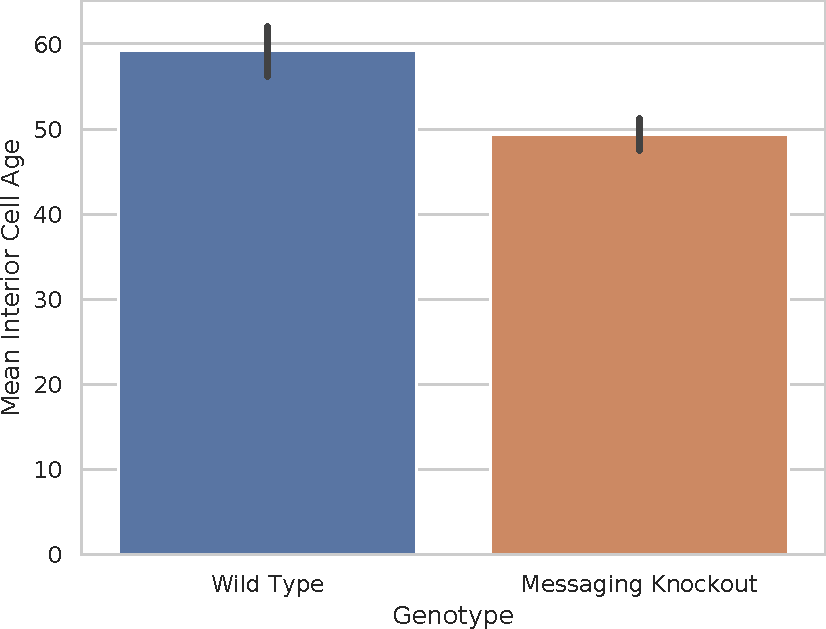
\includegraphics[width=\textwidth]{img/knockout/intermessaging-intergroup_border/title=cellageraw+_data_hathash_hash=ef9f5e984a40fbf6+_script_fullcat_hash=1faec38cdb6bd1de+_source_hash=53a2252-clean+ext=}%
% \caption{Interior cell age}
% \label{fig:intermessaging-intergroup_border-cellage}
% \end{minipage}
% \end{minipage}%
% \hspace*{\fill}

% \end{minipage}%
% \begin{minipage}[t]{\linewidth}
% \centering

% \hspace*{\fill}%
% \begin{minipage}[t]{0.8\linewidth}
% \centering
% \vspace{0pt} % for alignment
% \begin{minipage}[b]{\textwidth}
% \includegraphics[width=\textwidth]{img/knockout/intermessaging-intergroup_border/title=parentage+_data_hathash_hash=974d02d36b7dba1a+_script_fullcat_hash=7ee3d274683ffdb2+_source_hash=53a2252-clean+ext=}%
% \caption{Propagule parent age}
% \label{fig:intermessaging-intergroup_border-pparentage}
% \end{minipage}
% \end{minipage}%
% \hspace*{\fill}

% \vspace{1ex}

\hspace*{\fill}%
\begin{minipage}[t]{0.8\linewidth}
\centering
\vspace{0pt} % for alignment
\begin{minipage}[b]{\textwidth}
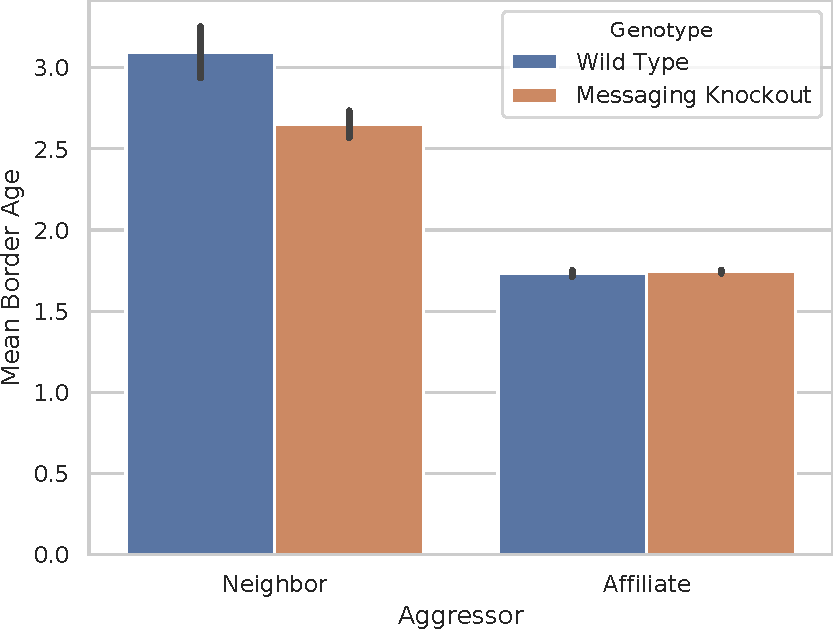
\includegraphics[width=\textwidth]{img/knockout/intermessaging-intergroup_border/title=comboborderage+_data_hathash_hash=8369fa84222d9217+_script_fullcat_hash=c576822d0876c8a8+_source_hash=53a2252-clean+ext=}\\
{\dissertationelse{(b)}{\textbf{(B)}} Border age}
% \label{fig:intermessaging-intergroup_border-borderage}
\end{minipage}
\end{minipage}%
\hspace*{\fill}

\vspace{1ex}

% \hspace*{\fill}%
% \begin{minipage}[t]{0.8\linewidth}
% \centering
% \vspace{0pt} % for alignment
% \begin{minipage}[b]{\textwidth}
% 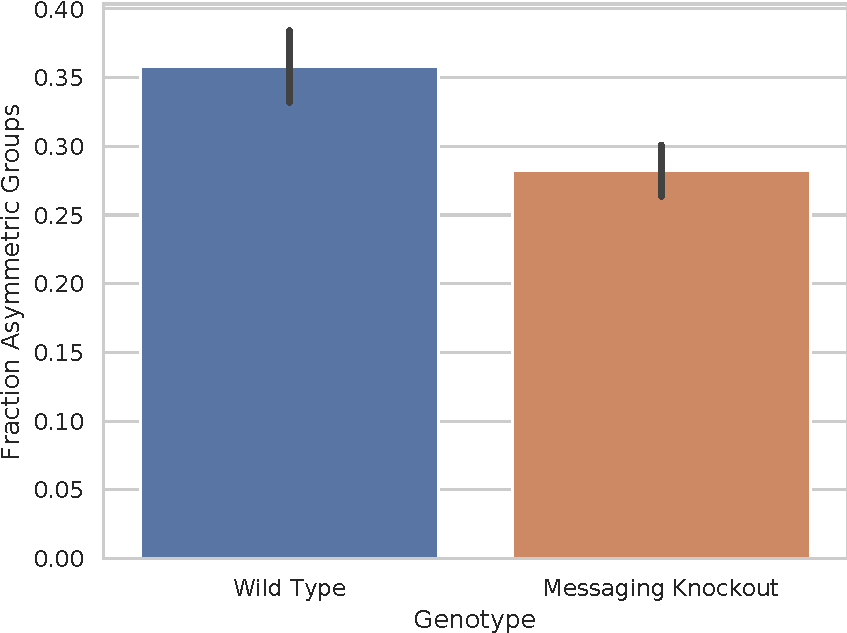
\includegraphics[width=\textwidth]{img/knockout/intermessaging-intergroup_border/title=metabolismasymmetry+_data_hathash_hash=3ce8f7b8474367f3+_script_fullcat_hash=0329612f3b158905+_source_hash=53a2252-clean+ext=}%
% \caption{Asymmetric border metabolism}
% \label{fig:intermessaging-intergroup_border-metabolism}
% \end{minipage}
% \end{minipage}%
% \hspace*{\fill}

\end{minipage}

\caption{
Comparison of wild type strain evolved under the ``Nested-Wave'' treatment and corresponding intercell messaging knockout strain.
Subfigure \dissertationelse{\ref{fig:ko-intermessaging-intergroup_border}a}{\textbf{(A)}} visualizes phenotypic traits in the wild type and knockout strain.
In the messaging visualization, color coding represents the volume of incoming messages.
White represents no incoming messages and the magenta to blue gradient runs from one incoming message to the maximum observed incoming message traffic.
In the resource sharing visualization, this same color coding represents the amount of incoming shared resource.
Solid black borders divide L1 hereditary groups and dotted light gray borders divide L0 hereditary groups.
Subfigure \dissertationelse{\ref{fig:ko-intermessaging-intergroup_border}b}{\textbf{(B)}} quantifies knockout effects on border age.
View an animation of the wild type strain at \url{https://hopth.ru/o}.
View the wild type strain in a live in-browser simulation at \url{https://hopth.ru/d}.
% minipages \ref{fig:intermessaging-intergroup_border-sharing}, \ref{fig:intermessaging-intergroup_border-cellage}, \ref{fig:intermessaging-intergroup_border-pparentage}, \ref{fig:intermessaging-intergroup_border-borderage}, and \ref{fig:intermessaging-intergroup_border-metabolism} quantify knockout effects on various phenotypic traits.
Error bars indicate 95\% confidence.
}
\label{fig:ko-intermessaging-intergroup_border}
% \end{minipage}

\end{center}
\end{figure}


Figure \ref{fig:ko-intermessaging-intergroup_border}\textbf{(A)} compares the cell-cell messaging, resource sharing, and parent-propagule phenotypes between wild type and cell-cell messaging knockout variants of a strain evolved under the Nested-Wave treatment.
Cell-cell messaging volume appears generally uniform in the interiors of hereditary groups, but some group-group borders --- largely, but not entirely parent-propagule interfaces --- manifest somewhat reduced cell-cell messaging overlaid with an alternating motif of elevated cell-cell messaging.
We affirmed the adaptiveness of cell-cell messaging in this strain through competition experiments between wild type and knockout variants ($19/20$; $p < 0.001$; two-tailed Binomial test).
The gene activated by cell-cell messaging in this strain contains a share resource instruction and, indeed, we observed significantly greater net resource sharing in the wild type strain
(%
WT: mean 0.27, S.D. 0.03, $n=20$;
KO: mean 0.23, S.D. 0.02, $n=20$;
$p < 0.001$, bootstrap test
%Figure \ref{fig:intermessaging-intergroup_border-sharing};
non-overlapping 95\% CI%
). %2020-01-06-ll.md
However, that same gene also contains a reproduction-inhibiting instruction, leading us to investigate whether cell-cell messaging could influence a broader set of phenotypic traits.

Cell-cell messaging in the wild type strain appears to be associated with a drawn out hereditary group life history.
The wild-type strain exhibits significantly greater mean cell age
(%
WT: mean 59, S.D. 7, $n=20$;
KO: mean 49, S.D. 4, $n=20$;
$p < 0.001$, bootstrap test%
%Figure \ref{fig:intermessaging-intergroup_border-sharing};
) %2020-01-06-ll.md
and, across propagule-generation events, significantly greater mean parent group age
(%
WT: mean 1055, S.D. 82, $n=20$;
KO: mean 924, S.D. 62, $n=20$;
$p < 0.001$, bootstrap test%
%Figure \ref{fig:intermessaging-intergroup_border-pparentage};
). %2020-01-06-ll.md
This strain exhibits the ``sweep'' life history depicted in Figure \ref{fig:lifecycle}\textbf{(C)}, so propagule generation can be largely or entirely destructive to the parent group.
So, the increase in mean cell age could plausibly be attributable to delayed propagule genesis or, alternatively, delayed propagule genesis could arise from other factors retarding life history.

In this strain, we anecdotally observed that contiguous bands of low cell turnover and anomalous cell-cell messaging volumes frequently arose along parent-propagule borders, but also occasionally between other pairs hereditary groups.
Cell-cell messaging not only enables functional coordination within cellular collectives but could also enable adaptive communication among cellular collectives.
This possibility motivated us to test for non-uniform interactions between hereditary groups that did not share a parent-propagule relationship.

We measured mean border age (equivalent to the youngest age of either flanking cell) along the borders of non-parent-propagule hereditary groups.
Figure \ref{fig:ko-intermessaging-intergroup_border}\textbf{(B)} splits this statistic out between borders that were disrupted either by cells birthed from members of the hereditary groups flanking the border (``affiliate'') or from a member of a third hereditary group (``neighbor'').
In both wild type and knockout strains, there was significantly more recent turnover in the absence of intrusion by a third hereditary group (non-overlapping 95\% CI, bootstrap test).
Restated, borders invaded by a third party were more on average more stable than those perturbed by either of the flanking hereditary groups.

This phenomenon was accentuated in the wild type strain.
Although the wild type strain exhibits slightly higher turnover rates on borders plied by only two groups, borders invaded by a third group are significantly more stale than the knockout strain (non-overlapping 95\% CI, bootstrap test).

Greater age of borders disrupted by a third party would be consistent with a general slowing of turnover as hereditary groups age or reduced resource availability in the presence of a third party.
However, a primitive tit-for-tat policy where a subset of non-parent-propagule hereditary group borders stabilize (until invaded by a third party) could also contribute to such an observation.

So, does the cell reproduction rate fluctuate uniformly across a hereditary group's borders or can reproduction rate differ significantly between a group's borders with different non-parent-propagule neighbor groups at a single time point?
To assess this question, we used Kruskal-Wallis tests (with Bonferroni correction) to screen for hereditary groups with border reproduction rate distributions that differed significantly between neighboring non-propagule-parent hereditary groups.
For each hereditary group, we calculated mean per-border-cell birth rate at the interface of each of its non-propagule-parent neighbor groups.
We collected observations with respect to each neighbor group every eighth update over 256 updates.
Groups with significantly differentiated border reproduction rate distributions occurred in both the wild type and messaging knockout strains.
That is, in both strains, we observed some groups that preferentially expended resource to reproduce at their interfaces with only certain non-parent-propagule hereditary group neighbors.

Again, this phenomenon was accentuated in the wild type strain.
A significantly higher proportion of groups exhibited asymmetric border reproduction rates with non-parent-child groups
(%
WT: mean 0.36, S.D. 0.06, $n=20$;
KO: mean 0.28, S.D. 0.04, $n=20$;
$p < 0.001$, bootstrap test%
). %2020-01-06-ll.md

Messaging between cells registered to different parent-propagule hereditary groups seems unlikely to directly underlie asymmetric border reproduction rates because execution of the gene targeted by messages triggers resource-sharing to the sender, which we seldom observed between non-parent-propagule groups (Figure \ref{fig:ko-intermessaging-intergroup_border}\textbf{(A)}).
So, intercell messaging within hereditary groups most likely underlies this phenomenon.
It seems most plausible that increased incidence of asymmetric border reproduction rates arises as a knock-on effect of the life history retardation effect originally discussed.
Perhaps older, ``full-grown'' hereditary groups arrive at a low-reproduction detente at interfaces with other older, ``full-grown'' hereditary groups while resisting incursion at interfaces with younger, growing hereditary groups.
This would constitute a contextually-expressed tit-for-tat policy, perhaps mediated by cell age or cell generations elapsed from the group's founding propagule cell.
